\documentclass[11pt,letterpaper]{article}
\usepackage[sinindice]{tecnm}
\usepackage{tikz}
\usetikzlibrary{arrows.meta,positioning}
\usepackage{graphicx}
\usepackage{booktabs,array,xcolor}
\usepackage{caption}

\materia{Inteligencia Artificial y su Ética}
\actividad{Tema 1.5 - Actividad 7 \\ Áreas Clave de la Inteligencia Artificial}
\profesor{M. Lilia Ureña Lugo}
% Agrega aquí el nombre completo del estudiante con la macro que use tu plantilla.

% Figura con imagen real; si el archivo aún no existe, muestra un recuadro
% para que el documento compile mientras consigues la imagen.
\newcommand{\figreal}[3]{% archivo, ancho, descripción
  \IfFileExists{#1}{\includegraphics[width=#2\textwidth]{#1}}%
  {\fbox{\parbox{#2\textwidth}{\centering\vspace{1.5cm}\small Insertar imagen: #3\vspace{1.5cm}}}}}

\begin{document}
\portada

%% ------------------------- CONTENIDO ---------------------------------

\section{Introducción}

La visión por computadora es el área de la Inteligencia Artificial que permite a una máquina interpretar imágenes y video para extraer información y tomar decisiones \parencite{iae_u1_diseno}. En este reporte se analizan cinco herramientas reales de esta área: qué hace cada una, qué problema del mundo actual resuelve y un caso concreto de aplicación. La Figura~\ref{fig:pipeline} resume el proceso general que siguen todas ellas.

\begin{figure}[ht]
\centering
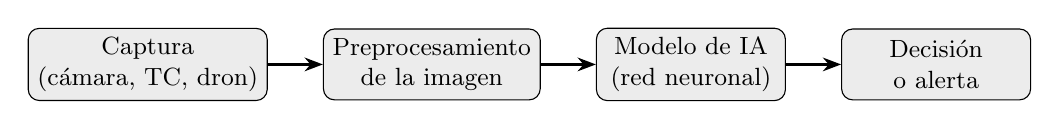
\begin{tikzpicture}[node distance=7mm, font=\small,
  box/.style={draw, rounded corners, fill=gray!15, minimum height=9mm, minimum width=24mm, align=center},
  arr/.style={-{Stealth}, thick}]
  \node[box] (a) {Captura\\(cámara, TC, dron)};
  \node[box, right=of a] (b) {Preprocesamiento\\de la imagen};
  \node[box, right=of b] (c) {Modelo de IA\\(red neuronal)};
  \node[box, right=of c] (d) {Decisión\\o alerta};
  \draw[arr] (a)--(b); \draw[arr] (b)--(c); \draw[arr] (c)--(d);
\end{tikzpicture}
\caption{Proceso general de un sistema de visión por computadora.}
\label{fig:pipeline}
\end{figure}

\section{Herramientas analizadas}

\subsection{Aidoc: diagnóstico médico por imágenes}

\textbf{Qué es.} Aidoc es una plataforma de IA que analiza estudios de radiología, como tomografías computarizadas (TC), y avisa al radiólogo cuando detecta posibles hallazgos urgentes \parencite{aidoc_fda}. Cuenta con autorizaciones de la FDA de Estados Unidos para priorización (\textit{triage}) en TC, entre ellas hemorragia intracraneal y embolia pulmonar.

\textbf{Problema que resuelve.} En urgencias, un estudio crítico puede esperar horas en la lista de lectura. El sistema reordena la lista para que los casos sospechosos se revisen primero.

\textbf{Caso concreto.} Se realiza una TC de cráneo a un paciente con golpe en la cabeza. Aidoc analiza el estudio y, si detecta una posible hemorragia intracraneal, notifica al radiólogo y sube ese estudio en su lista de prioridad. El diagnóstico final lo sigue emitiendo el médico.

\begin{figure}[ht]
\centering
\figreal{img/aidoc.png}{0.62}{captura o imagen oficial de Aidoc (aidoc.com)}
\caption{Aidoc: notificación de hallazgo sospechoso en una TC. Fuente: \textcite{aidoc_fda}.}
\label{fig:aidoc}
\end{figure}

\subsection{Cognex VisionPro Deep Learning: inspección de calidad industrial}

\textbf{Qué es.} Software de Cognex que usa aprendizaje profundo para detectar defectos, verificar ensambles, clasificar piezas y leer texto (OCR) en líneas de producción \parencite{cognex_dl}. Se entrena con imágenes de ejemplo de piezas buenas y defectuosas.

\textbf{Problema que resuelve.} La inspección visual humana es lenta, costosa y se ve afectada por la fatiga. Defectos difíciles de describir con reglas fijas, como rayones o variaciones en superficies, pasan sin detectarse y generan desperdicio y devoluciones.

\textbf{Caso concreto.} En una línea que fabrica tarjetas electrónicas, una cámara fotografía cada pieza; el modelo entrenado marca las que presentan soldaduras defectuosas o componentes faltantes y las separa antes del empaque.

\begin{figure}[ht]
\centering
\figreal{img/cognex.png}{0.7}{imagen oficial de Cognex mostrando detección de defectos}
\caption{Detección de defectos con aprendizaje profundo. Fuente: \textcite{cognex_dl}.}
\label{fig:cognex}
\end{figure}

\subsection{Tesla Vision: percepción para vehículos autónomos}

\textbf{Qué es.} Sistema de percepción de Tesla basado en ocho cámaras que dan visibilidad de 360 grados hasta unos 250 metros, procesadas por redes neuronales \parencite{tesla_vision}. Tesla dejó de usar radar y sensores ultrasónicos en sus vehículos nuevos y depende solo de cámaras.

\textbf{Problema que resuelve.} Los accidentes viales suelen deberse a distracción o cansancio. El sistema identifica vehículos, peatones, carriles y señales de forma continua y alimenta funciones de asistencia a la conducción como Autopilot.

\textbf{Caso concreto.} En carretera, las cámaras detectan el carril y al vehículo de adelante; el sistema mantiene el vehículo dentro del carril y ajusta la velocidad para conservar la distancia.

\begin{figure}[ht]
\centering
\figreal{img/teslavision.jpg}{0.7}{imagen oficial de Tesla con la cobertura de las ocho cámaras}
\caption{Cobertura de cámaras de Tesla Vision. Fuente: \textcite{tesla_vision}.}
\label{fig:tesla}
\end{figure}

\subsection{Adobe Firefly y Generative Fill: generación y edición de imágenes}

\textbf{Qué es.} Firefly es la familia de modelos generativos de Adobe. En Photoshop, la función Generative Fill permite agregar, extender o quitar elementos de una imagen escribiendo una instrucción de texto, sin alterar la imagen original porque el resultado se guarda en capas generativas \parencite{adobe_firefly}.

\textbf{Problema que resuelve.} Producir y retocar material gráfico requiere mucho tiempo y personal especializado. Esta herramienta reduce el tiempo de edición y de prototipado visual.

\textbf{Caso concreto.} Un diseñador de una tienda en línea necesita ampliar el fondo de una fotografía de producto para un banner; selecciona el área, escribe lo que desea y el sistema genera la extensión con luz y perspectiva coherentes.

\begin{figure}[ht]
\centering
\figreal{img/adobefirefly.jpeg}{0.55}{ejemplo oficial de Generative Fill (antes y después)}
\caption{Ejemplo de Generative Fill en Photoshop. Fuente: \textcite{adobe_firefly}.}
\label{fig:firefly}
\end{figure}

\subsection{John Deere See \& Spray: agricultura de precisión}

\textbf{Qué es.} Sistema de John Deere con cámaras montadas en el aspersor de la maquinaria, que distinguen en tiempo real la maleza del cultivo y aplican herbicida solo sobre la maleza \parencite{deere_2024}.

\textbf{Problema que resuelve.} Aplicar herbicida en todo el campo es costoso y contamina. Deere reportó un ahorro promedio de herbicida de 59\,\% en 2024 frente a la aspersión generalizada \parencite{deere_2024} y cercano a 50\,\% en 2025, con más de cinco millones de acres \parencite{deere_2025}. Son cifras de la propia empresa y dependen de las condiciones de cada campo.

\textbf{Caso concreto.} Un agricultor de soya recorre su parcela con el aspersor; las cámaras detectan la maleza entre las hileras y solo se activan las boquillas sobre ella, lo que reduce el producto usado.

\begin{figure}[ht]
\centering
\figreal{img/JohnDeereSeeSpray.jpg}{0.6}{imagen oficial de See \& Spray (deere.com)}
\caption{Aspersor con See \& Spray. Fuente: \textcite{deere_2024}.}
\label{fig:seespray}
\end{figure}

\section{Comparación}

\begin{table}[ht]
\centering\small
\renewcommand{\arraystretch}{1.2}
\begin{tabular}{>{\raggedright\arraybackslash}p{2.9cm}>{\raggedright\arraybackslash}p{3.4cm}>{\raggedright\arraybackslash}p{3.6cm}>{\raggedright\arraybackslash}p{3.4cm}}
\toprule
\textbf{Herramienta} & \textbf{Sector} & \textbf{Problema} & \textbf{Resultado} \\
\midrule
Aidoc & Salud & Retraso en estudios urgentes & Priorización de casos críticos \\
Cognex VisionPro DL & Manufactura & Defectos y fatiga en inspección & Detección automática de fallas \\
Tesla Vision & Transporte & Errores por distracción & Asistencia a la conducción \\
Adobe Firefly & Diseño y medios & Costo y tiempo de edición & Edición con texto en segundos \\
John Deere See \& Spray & Agricultura & Exceso de herbicida & Ahorro de 50--59\,\% (según Deere) \\
\bottomrule
\end{tabular}
\caption{Resumen de las herramientas analizadas. Elaboración propia.}
\label{tab:resumen}
\end{table}

\section{Conclusión}

Las cinco herramientas muestran que la visión por computadora ya se usa en sectores muy distintos. En todos los casos la IA no sustituye por completo a la persona: apoya al radiólogo, al inspector, al conductor, al diseñador o al agricultor, y reduce tiempo, costos o riesgos. Los beneficios que reportan las empresas deben tomarse con cuidado, porque provienen de los propios fabricantes.

\referencias
\end{document}
